%!TEX TS-program = xelatex
\documentclass[]{friggeri-cv}
\usepackage{afterpage}
\usepackage{hyperref}
\usepackage{color}
\usepackage{xcolor}
\usepackage{smartdiagram}
\usepackage{fontspec}
% if you want to add fontawesome package
% you need to compile the tex file with LuaLaTeX
% References:
%   http://texdoc.net/texmf-dist/doc/latex/fontawesome/fontawesome.pdf
%   https://www.ctan.org/tex-archive/fonts/fontawesome?lang=en
%\usepackage{fontawesome}
\usepackage{metalogo}
\usepackage{dtklogos}
\usepackage[utf8]{inputenc}
\usepackage{tikz}
\usetikzlibrary{mindmap,shadows}
\hypersetup{
    pdftitle={},
    pdfauthor={},
    pdfsubject={},
    pdfkeywords={},
    colorlinks=false,           % no lik border color
    allbordercolors=white       % white border color for all
}
\smartdiagramset{
    bubble center node font = \footnotesize,
    bubble node font = \footnotesize,
    % specifies the minimum size of the bubble center node
    bubble center node size = 0.5cm,
    %  specifies the minimum size of the bubbles
    bubble node size = 0.5cm,
    % specifies which is the distance among the bubble center node and the other bubbles
    distance center/other bubbles = 0.3cm,
    % sets the distance from the text to the border of the bubble center node
    distance text center bubble = 0.5cm,
    % set center bubble color
    bubble center node color = pblue,
    % define the list of colors usable in the diagram
    set color list = {lightgray, materialcyan, orange, green, materialorange, materialteal, materialamber, materialindigo, materialgreen, materiallime},
    % sets the opacity at which the bubbles are shown
    bubble fill opacity = 0.6,
    % sets the opacity at which the bubble text is shown
    bubble text opacity = 0.5,
}

\addbibresource{bibliography.bib}
\RequirePackage{xcolor}
\definecolor{pblue}{HTML}{0395DE}

\begin{document}
\header{Artyom}{Solovyov}
      {Principal Software Engineer}
      
% Fake text to add separator      
\fcolorbox{white}{gray}{\parbox{\dimexpr\textwidth-2\fboxsep-2\fboxrule}{%
.....
}}

% In the aside, each new line forces a line break
\begin{aside}
  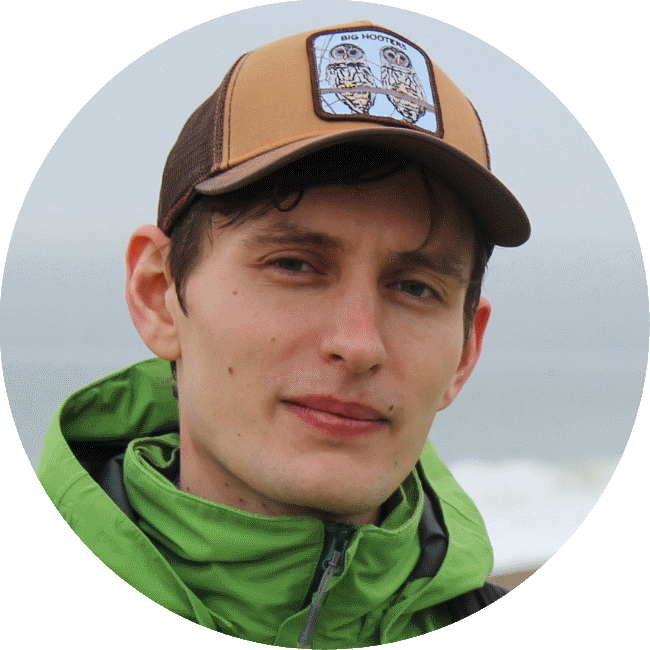
\includegraphics[scale=0.18]{img/ava.png}
  \section{Address}
    Spain, Valencia
    ~
  \section{Telephone}
    +34 636 485 268
    ~
  \section{Mail}
    \href{mailto:tema.solovyov@gmail.com}{\textbf{tema.solovyov@}\\gmail.com}
    ~
  \section{LinkedIn}
    \href{https://www.linkedin.com/in/temasolovyov}{temasolovyov}
    ~
  \section{GitHub}
    \href{https://github.com/mobichel}{github.com/mobichel}
    ~
    \section{Skills}
    \smartdiagram[bubble diagram]{
        \textbf{JavaScript},
        \textbf{TypeScript},
        \textbf{Java},
        \textbf{k8s/Helm},
        \textbf{Git/Hg},
        \textbf{Bash},
        \textbf{Maven},
        \textbf{Node.js},
        \textbf{HTML/CSS},
        \textbf{Angular},
        \textbf{Spring}
    }
    ~
    \section{Languages}
        \textbf{Russian}
\includegraphics[scale=0.40]{img/5stars.png}
        \textbf{English}
\includegraphics[scale=0.40]{img/4stars.png}
        \textbf{Español}
\includegraphics[scale=0.40]{img/1stars.png}
    ~
\end{aside}
~
\section{Experience}
\begin{entrylist}
  \entry
    {09/22 - now}
    {Principal Software Engineer - Team Lead\\}
    {\href{http://www.genesys.com/}{Genesys, Spain}}
    {Continue to work on Genesys reporting projects as a Team Lead: \\
    - Manage a small size team of developers distributed around the globe. \\
    - Individual contribution into Genesys Pulse product as Java/JavaScript developer. \\
    - Continuously support the Genesys Pulse product by providing security updates and implementing customers requests. \\}
    \entry
    {05/18 - 06/22}
    {Principal Software Engineer - Team Lead\\}
    {\href{http://www.genesys.com/}{Genesys, Russia}}
    {Continue to work on Genesys Pulse project as a Team Lead: \\
    - Manage a small size team of front-end developers. \\
    - Perform a migration to latest Angular versions. \\
    - Migrated to Angular CLI as a main build tool. \\
    - Build a proof of concept for AWS Lambda powered back-end replacement. \\}
    \entry
    {05/16 - 04/18}
    {Staff Software Engineer\\}
    {\href{http://www.genesys.com/}{Genesys, Russia}}
    {Continued to work on Genesys Pulse project. \\
    - Developed new features. \\
    - Implemented plug-in system to allow users develop own chart types and use them in Genesys Pulse. \\
    - Migrated existing code base to ES6 using Babel transpiler, reworked build pipeline to use Gulp and Webpack.\\}
    \entry
    {05/15 - 04/16}
    {Senior Software Engineer\\}
    {\href{http://www.genesys.com/}{Genesys, Russia}}
    {Worked as a full-stack developer on Genesys Pulse project. \\
    - Developed new features. \\
    - Performed migration from Backbone to AngularJS 1.x. \\
    - Reworked storage layer as independent module for further reusing in other project components (Java, JOOQ).\\}
    \entry
    {10/11 - 04/15}
    {Software Engineer\\}
    {\href{http://www.genesys.com/}{Genesys, Russia}}
    {Worked as a full-stack developer on Genesys Pulse a real-time web based reporting system. \\
    - Participated in design and development of back-end part (Java, Spring). \\
    - Implemented serialization library for marshaling and unmarshaling Google Protocol Buffers objects to JSON and vise versa. \\
    - Developed front-end part with JavaScript, Backbone and in-company developed widget library. \\
    - Implemented push notifications using CometD and RabbitMQ as a message broker.\\
    - Contributed into in-company developed widget library.\\}
    
\end{entrylist}

\newpage
\section{Experience}
\begin{entrylist}
\entry
    {02/08 - 10/11}
    {Software Engineer\\}
    {\href{http://nicetu.spb.ru/index.php/en}{Research and Engineering Center of St. Petersburg Electrotechnical University, Russia}}
    {Worked on various projects: \\
    - Developed tool for visualization and analysis of telemetry information (Java, Swing) \\
    - Participated in design and implementation of the scheduling system (Java, Swing, Google Protocol Buffers, ActiveMQ) \\
    - Improved automated functional testing system.}
\end{entrylist}

\section{Education}
\begin{entrylist}
  \entry
    {2009 - 2011}
    {Master's Degree in Computer Systems Engineering and Informatics.\\}
    {\href{http://www.eltech.ru/en/}{St. Petersburg Electrotechnical University}}
    {Faculty of Computer Science and Technology. Department of Software Engineering and Computer Applications. Specialization in Software Development Technologies\\}
  \entry
    {2005 - 2009}
    {Bachelor's Degree in Computer Systems Engineering and Informatics\\}
    {\href{http://www.eltech.ru/en/}{St. Petersburg Electrotechnical University}}
    {Faculty of Computer Science and Technology. Department of Software Engineering and Computer Applications.\\}
\end{entrylist}

\section{Honors \& Awards}
\begin{entrylist}
  \entry
    {2019}
    {Genesys Hackathon Award - Best Project and Science Booth}{}{}
\end{entrylist}

\begin{entrylist}
  \entry
    {2014}
    {Genesys Appreciation Award}{}{}
\end{entrylist}

\begin{entrylist}
  \entry
    {2013}
    {Genesys Photo Contest Award}{}{}
\end{entrylist}

\section{Personal Info}
\emph{I'm a goal oriented strong team player, curious explorer and traveler, eager to learn and open to new technologies.}

\end{document}
